\section{Experiments}\label{sec:experiments}
We demonstrate Meta-MAPG's efficacy on a diverse suite of domains, including the full spectrum of mixed incentive, competitive, and cooperative settings. 
% We first explain our setup for meta-learning in multiagent learning settings, and then evaluate Meta-MAPG's adaptation performance in various aspects, including its sample complexity, generalization to out of distribution, and ablation analysis.
The code is available at \url{https://git.io/JZsfg}, and video highlights are available at \url{http://bit.ly/2L8Wvch}. 
The mean and 95\% confidence interval computed for 10 seeds are shown in each figure.

\subsection{Experimental Setup for Meta-Learning in MARL}
\noindent\header{Training protocol.}
In our experiments, we evaluate a meta-agent $i$'s adaptability with respect to a peer agent $j$ learning in the environment. 
Specifically, agent $j$ is sampled from a population of initial peer policy parameters $p(\bm{\phi}^{\bm{-i}}_{\bm{0}})$. Then, both agents adapt their behavior following the policy gradient with a linear feature baseline~\citep{duan-16-linearbaseline} (see~\cref{fig:meta-learning-setup}). 
Importantly, the population captures diverse behaviors of $j$, such as varying expertise in solving a task, and $j$'s initial policy is hidden to $i$. 
Hence, a meta-agent $i$ should: 1) adapt to a differently initialized agent $j$ with varying behaviors and 2) continuously adapt with respect to $j$'s changing policy.

During meta-training, a meta-agent $i$ interacts with peers drawn from the distribution and optimizes its initial policy parameters $\phi^{i}_{0}$.
At the end of meta-training, a new peer $j$ is sampled from the distribution, and we measure $i$'s performance throughout the Markov chain.
%%%%%%%%%%%%%%%%%%%%%%%%%%%%%%%%%%%%%%%%%%%%%%%%%%%%%%%%%%%%%%%%%%%%%%%%%%%%%%%%%
\begin{figure}[t]
    \centering
    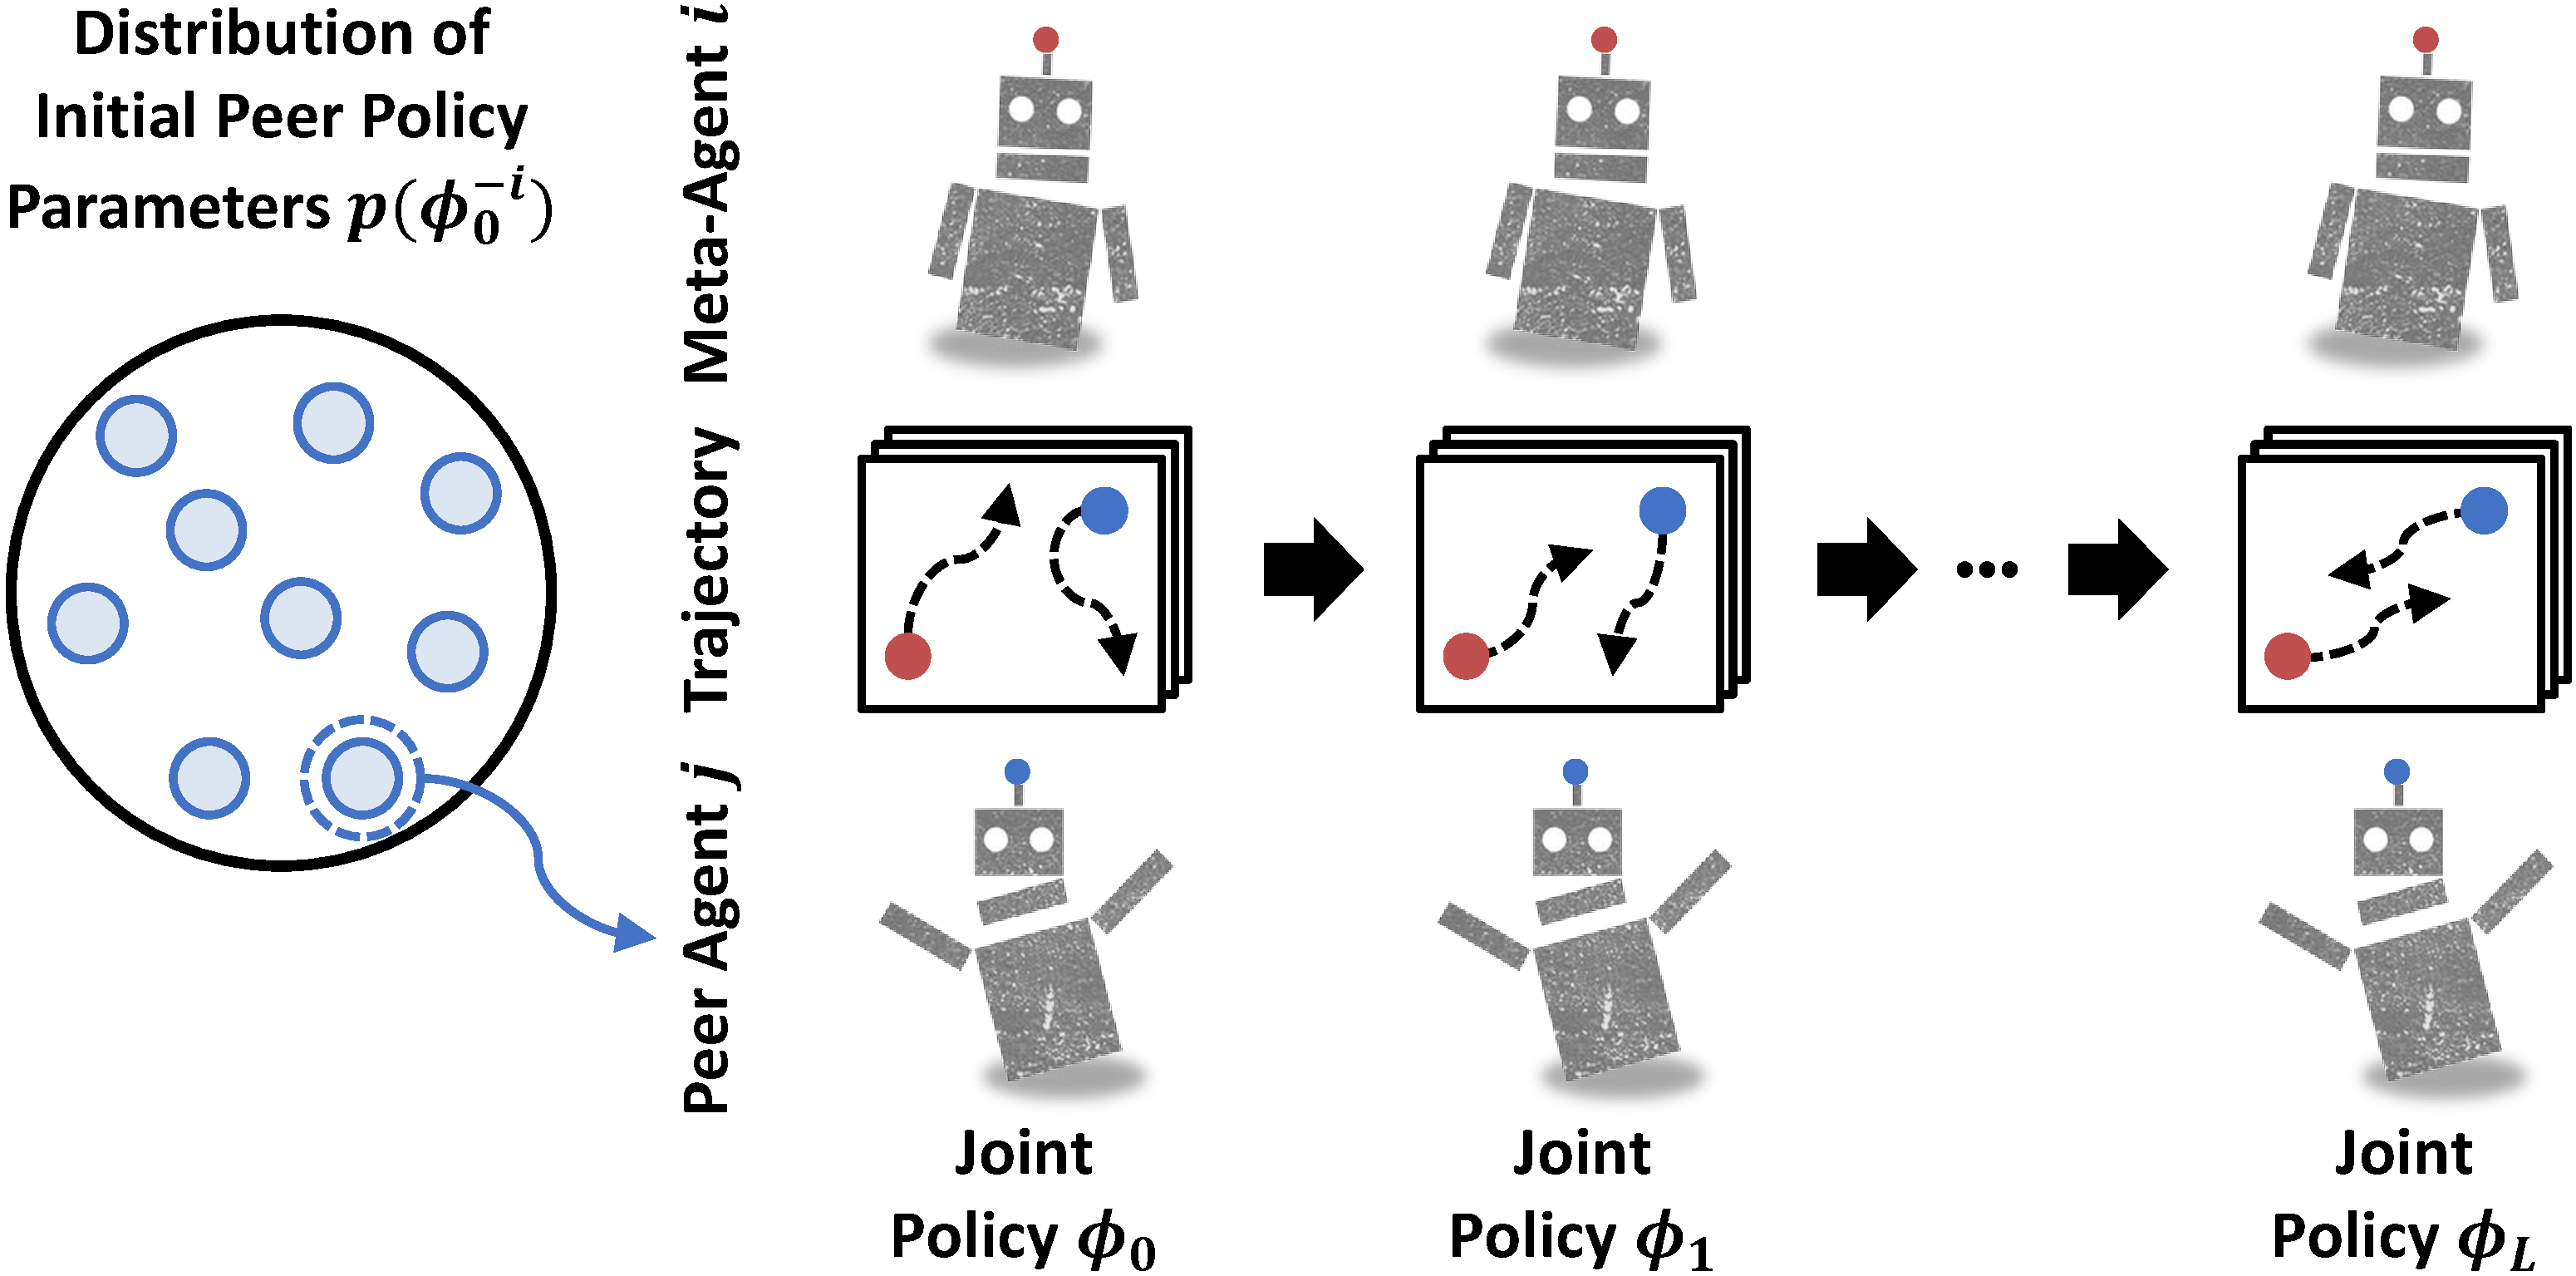
\includegraphics[height=3.7cm]{figs/experimental_setup_v2.pdf}
    \vspace{-0.3cm}
    \caption{Experimental setup for meta-learning. A peer $j$'s policy is initialized randomly from a population $p(\bm{\phi}^{\bm{-i}}_{\bm{0}})$ and is updated based on the policy gradient optimization, requiring a meta-agent $i$ to adapt to differently initialized $j$ and its changing policy.}
    \label{fig:meta-learning-setup}
    \vskip-0.16in
\end{figure}
%%%%%%%%%%%%%%%%%%%%%%%%%%%%%%%%%%%%%%%%%%%%%%%%%%%%%%%%%%%%%%%%%%%%%%%%%%%%%%%%%

\noindent\header{Adaptation baselines.}
We compare Meta-MAPG with the following baseline adaptation strategies for an agent $i$:
\begin{enumerate}[wide, labelindent=0pt, label=\arabic*), topsep=0pt]
    \itemsep 0pt
    \item Meta-PG~\citep{alshedivat2018continuous}: A meta-learning approach that only considers how to improve its own learning. We detail our implementation of Meta-PG and a low-level difference with the original method in~\cref{sec:meta-pg-difference-details}.
    \item LOLA-DiCE~\citep{foerster2018dice}: 
    An approach that only considers how to shape the learning dynamics of other agents in the environment through the Differentiable Monte-Carlo Estimator (DiCE) operation. Note that LOLA-DiCE is an extension of the original LOLA approach.
    \item REINFORCE~\citep{Williams1992}: A simple policy gradient approach that considers neither an agent's own learning nor the learning processes of other agents. This baseline represents multiagent approaches that assume each agent leverages a stationary policy in the future. 
\end{enumerate}

\noindent\header{Implementation.}
We implement each adaptation method's policy leveraging an LSTM and use the generalized advantage estimation~\citep{schulmanetal-16-gae} with a learned value function for the meta-optimization. 
We also apply DiCE during the inner-loop optimization~\citep{foerster2018dice} to compute the peer learning gradients, and we learn dynamic inner-loop learning rates during meta-training as suggested in~\citet{alshedivat2018continuous}.
We refer to Appendices E, F, G, I for the remaining details including hyperparameters.

\noindent\header{Experiment complexity.} 
We study various aspects of Meta-MAPG based on two repeated matrix games (see \Cref{tab:ipd-payoff-table,tab:rps-payoff-table}). 
We note that the repeated matrix domains we consider match the environment complexity of previous work on the topic of peer learning awareness in MARL~\citep{foerster17lola,foerster2018dice,letcher2018stable}.
We also considered the RoboSumo domain from~\citet{alshedivat2018continuous}. 
However, the training performance was very sensitive to the relative weights between the shaped reward functions and we could not reproduce the results from~\citet{alshedivat2018continuous} with the default weights.
Instead, we experimented with another challenging environment leveraging the multi-agent MuJoCo benchmark~\citep{dewitt2020deep_multimujoco} to demonstrate the scability of Meta-MAPG.
% We also consider a multiagent-MuJoCo benchmark~\citep{dewitt2020deep_multimujoco} and show that Meta-MAPG can be scaled to a complex domain. 
Specifically, the environment shown in~\Cref{fig:multi-mujoco-domain} has high complexity: 1) the domain has continuous and large observation/action spaces, and 2) the agents are coupled within the same robot, resulting in a more challenging control problem than controlling the robot alone with full autonomy.
% requires close cooperation and coordination between them.
% We also consider a variant of a repeated matrix game with more than $2$ agents, where the domain becomes harder because the state space dimension grows exponentially as a function of the number of agents and a meta-agent $i$ needs to consider more peers in the process of affecting their future policies. 
%%%%%%%%%%%%%%%%%%%%%%%%%%%%%%
\begin{figure}[t!]
\captionsetup[subfigure]{skip=0pt}
    \begin{subfigure}[b]{0.49\linewidth}
        \centering
        \footnotesize
        \resizebox{0.9\textwidth}{!}{
        \setlength{\tabcolsep}{2pt}
        \begin{tabular}[b]{cc|cc}
        \multicolumn{2}{c}{} & \multicolumn{2}{c}{Agent $j$}\\
        \parbox[t]{3mm}{\multirow{3}{*}{\rotatebox[origin=c]{90}{Agent $i$}}} 
            &       & $C$       & $D$       \\\cline{2-4}
        \rule{0pt}{3pt}    & $C$   & $(0.5,0.5)$ & $(\text{-}1.5,1.5)$  \\
            & $D$   & $(1.5,\text{-}1.5)$  & $(\text{-}0.5,\text{-}0.5)$ 
        \end{tabular}}
        \caption{IPD payoff table}
        \label{tab:ipd-payoff-table}
    \end{subfigure}
    \begin{subfigure}[b]{0.49\linewidth}
        \centering
        \footnotesize
        \resizebox{0.9\textwidth}{!}{
        \setlength{\tabcolsep}{2pt}
        \begin{tabular}{cc|ccc}
        \multicolumn{2}{c}{} & \multicolumn{3}{c}{Agent $j$}\\
        \parbox[t]{3mm}{\multirow{3}{*}{\rotatebox[origin=c]{90}{Agent $i$}}} 
            &       & $R$       & $P$ & $S$      \\\cline{2-5}
        \rule{0pt}{3pt}    & $R$   & $(0,0)$   & $(\text{-}1,1)$ & $(1,\text{-}1)$ \\
            & $P$   & $(1,\text{-}1)$  & $(0,0)$ & $(\text{-}1,1)$ \\
            & $S$   & $(\text{-}1,1)$  & $(1,\text{-}1)$ & $(0,0)$
        \end{tabular}}
        \caption{RPS payoff table}
        \label{tab:rps-payoff-table}
    \end{subfigure}
    \begin{subfigure}[b]{\linewidth}
        \centering
        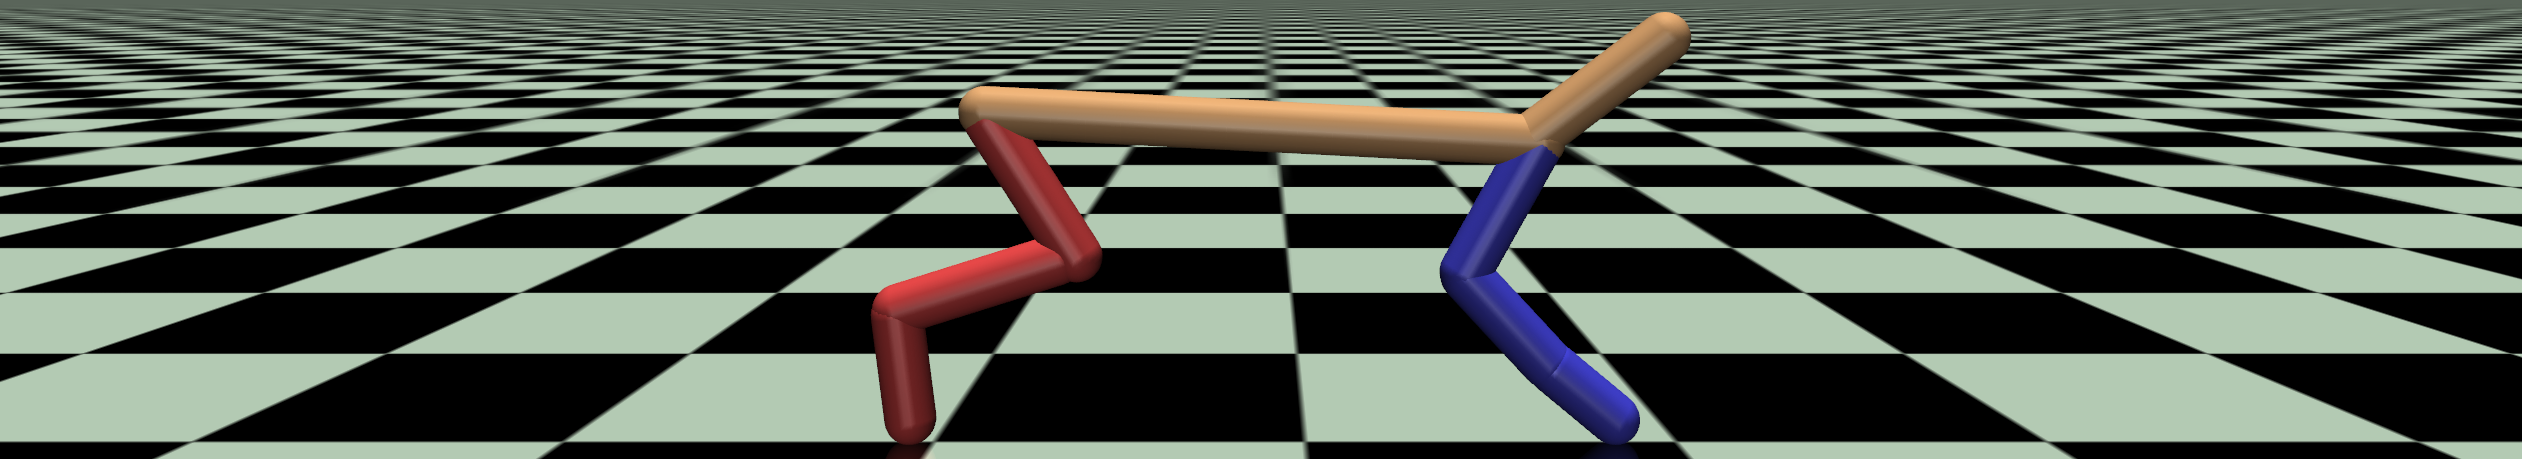
\includegraphics[trim=100 0 0 0,clip, height=1.35cm]{figs/half_cheetah_v3.png}
        \caption{2-Agent HalfCheetah Benchmark}
        \label{fig:multi-mujoco-domain}
    \end{subfigure}
    \vspace{-0.74cm}
    \caption{\textbf{(a)} IPD payoff table. \textbf{(b)} RPS payoff table. \textbf{(c)} $2$-Agent HalfCheetah benchmark, where two agents are coupled within the robot and control the robot together: the red and blue agent control three joints of the back and front leg, respectively.}
    \vskip-0.2in
\end{figure}
%%%%%%%%%%%%%%%%%%%%%%%%%%%%%%

%%%%%%%%%%%%%%%%%%%%%%%%%%%%%%
\begin{figure*}[t!]
\captionsetup[subfigure]{skip=0pt, aboveskip=9pt}
    \begin{subfigure}[b]{0.247\linewidth}
        \centering
        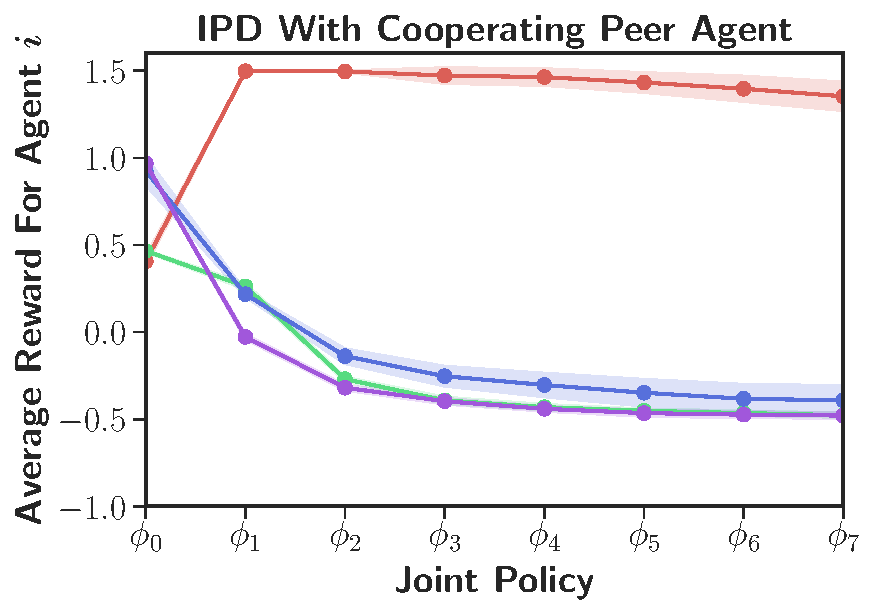
\includegraphics[height=2.9cm]{figs/ipd_cooperative.pdf}
        \caption{}
        \label{fig:ipd-cooperative-result}
    \end{subfigure}
    \begin{subfigure}[b]{0.247\linewidth}
        \centering
        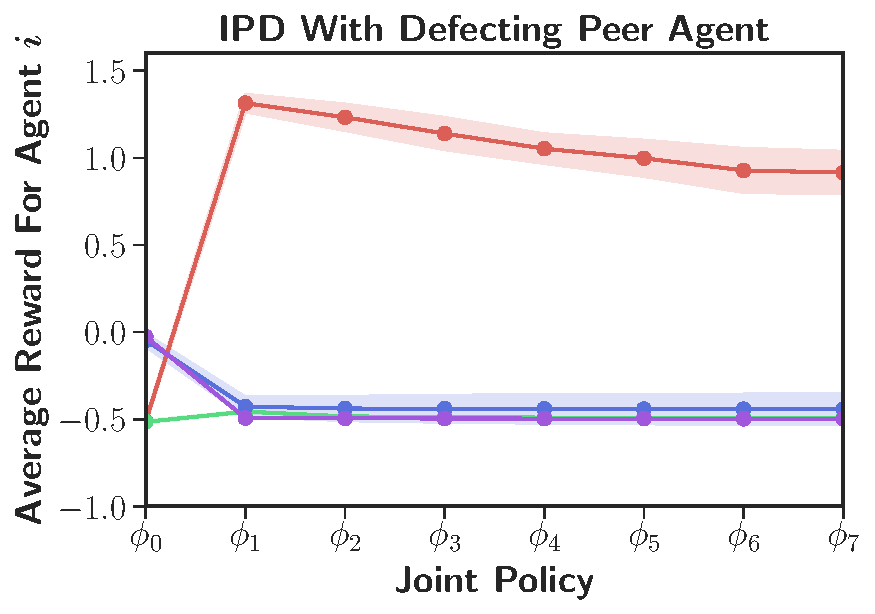
\includegraphics[height=2.9cm]{figs/ipd_defective.pdf}
        \caption{}
        \label{fig:ipd-defective-result}
    \end{subfigure}
    \begin{subfigure}[b]{0.247\linewidth}
        \centering
        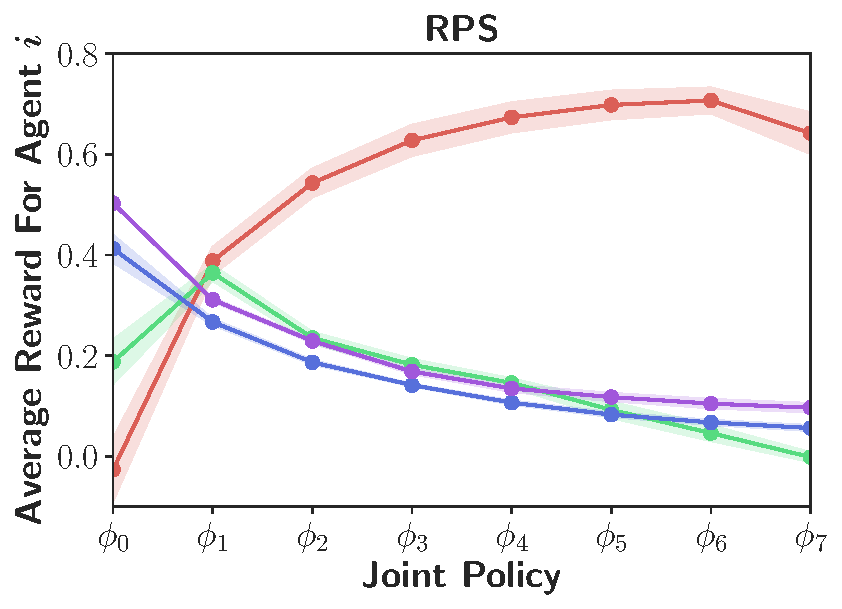
\includegraphics[height=2.9cm]{figs/rps.pdf}
        \caption{}
        \label{fig:rps-result}
    \end{subfigure}
    \begin{subfigure}[b]{0.247\linewidth}
        \centering
        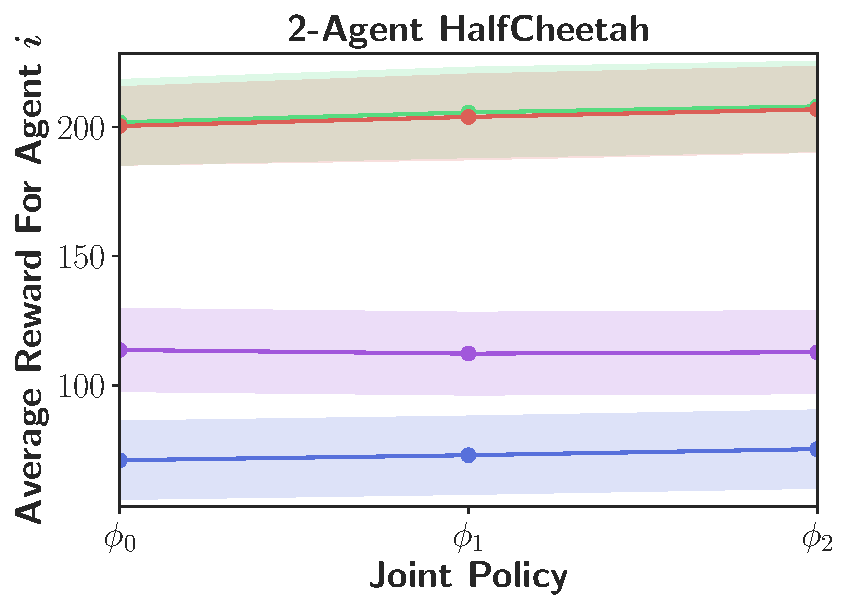
\includegraphics[height=2.9cm]{figs/halfcheetah_result.pdf}
        \caption{}
        \label{fig:halfcheeta-result-finale}
    \end{subfigure}
    
    \vspace{-0.9cm}
    \begin{subfigure}[b]{\linewidth}
        \centering
        
\includegraphics[height=0.13cm]{figs/legend.pdf}
    \end{subfigure}
    \caption{Adaptation performance during meta-testing in mixed incentive ((\textbf{a}) and (\textbf{b})), competitive (\textbf{c}), and cooperative (\textbf{d}) environments. 
    The results show that Meta-MAPG can successfully adapt to a new and learning peer agent throughout the Markov chain. 
    }
    \vskip-0.17in
\end{figure*}
%%%%%%%%%%%%%%%%%%%%%%%%%%%%%%

\subsection{IPD Environment: Mixed Incentive}
\begin{question}
Is it essential to consider both an agent's own learning and the learning of others? \\[-2em]
\end{question}
To address this question, we consider the classic iterated prisoner's dilemma (IPD) domain. 
In IPD, agents $i$ and $j$ act by either (C)ooperating or (D)efecting and receive rewards according to the mixed incentive payoff defined in~\cref{tab:ipd-payoff-table}. 
As in~\citet{foerster17lola}, we model the state space as $s_{0}\!=\!\varnothing$ and $s_{t}\!=\!\bm{a}_{\bm{t-1}}$ for $t\geq1$.
For meta-learning, we construct a population of initial personas $p(\bm{\phi}^{\bm{-i}}_{\bm{0}})$ that include cooperating personas (i.e., having a probability of cooperating between $0.5$ and $1.0$ at any state) and defecting personas (i.e., having a probability of cooperating between $0$ and $0.5$ at any state).
\cref{fig:ipd-pca} in Appendix shows the population distribution utilized for training and evaluation.
% A peer agent $j$ is initialized randomly from the population and adapts its behavior based on the policy gradient optimization throughout the Markov chain.
% Hence, an agent $i$ should: 1) adapt to a differently initialized agent $j$ with varying amounts of cooperation, and 2) continuously adapt with respect to the learning of $j$. 

The adaptation performance during meta-testing when an agent $i$, meta-trained with either Meta-MAPG or the baseline methods, interacts with an initially cooperating or defecting agent $j$ is shown in~\Cref{fig:ipd-cooperative-result} and~\Cref{fig:ipd-defective-result}, respectively.
In both cases, our meta-agent successfully infers the underlying persona of $j$ and adapts throughout the Markov chain obtaining higher rewards than the baselines. 
We observe that performance generally decreases as the number of joint policy updates increases across all adaptation methods. 
This decrease in performance is expected as each model is playing with another reasonable agent that is also constantly learning. 
As a result, $j$ realizes it could potentially achieve more reward by defecting more often.
Hence, to achieve good adaptation performance in IPD, an agent $i$ should attempt to shape $j$'s future policies toward staying cooperative as long as possible such that $i$ can take advantage, which is achieved by accounting for both an agent's own learning and the learning of other peer agents in Meta-MAPG. 

We explore each adaptation method in more detail by visualizing the action probability dynamics throughout the Markov chain. In general, we observe that the baseline methods have converged to initially defecting strategies, attempting to get larger rewards than a peer agent $j$ in the first trajectory $\tau_{\bm{\phi}_{\bm{0}}}$.
While this strategy can result in better initial performance than $j$, the peer agent will quickly change its policy so that it is defecting with high probability as well (see~\cref{fig:ipd-meta-pg-analysis,fig:ipd-dice-analysis,fig:ipd-reinforce-analysis} in Appendix). 
By contrast, our meta-agent learns to act cooperatively in $\tau_{\bm{\phi}_{\bm{0}}}$ and then take advantage by deceiving agent $j$ as it attempts to cooperate at future steps (see~\cref{fig:ipd-meta-mapg-analysis} in Appendix).

\begin{question}
How is adaptation performance affected by the number of trajectories between changes? \\[-2em]
\end{question}
We control the level of non-stationarity by adjusting the number of trajectories $K$ between updates (refer to~\Cref{sec:markov-chain-of-policies}). 
The results in~\cref{fig:sample-complexity} shows that the area under the curve (AUC) (i.e., the reward summation during $\bm{\phi}_{\bm{1:L}}$) generally decreases when $K$ decreases in IPD. 
This result is expected since the inner-loop updates are based on the policy gradient, which can suffer from a high variance. 
Thus, with a smaller batch size, policy updates have a higher variance and lead to noisier policy updates. As a result, it is harder to anticipate and influence the future policies of peers. 
Nevertheless, Meta-MAPG achieves the best AUC in all cases.

\begin{question}
How does Meta-MAPG perform with decentralized meta-training?
\\[-2em]
\end{question}
We compare the performance of Meta-MAPG with and without opponent modeling (OM) in~\cref{fig:ipd-om}.
We note that Meta-MAPG with opponent modeling can infer policy parameters for peer agents and compute the peer learning gradient in a decentralized manner, performing better than the Meta-PG baseline.
However, opponent modeling introduces noise in predicting the future policy parameters of peer agents because the parameters must be inferred by observing the actions they take alone without any supervision about the parameters themselves. 
Thus, as expected, a meta-agent experiences difficulty in correctly considering the learning process of a peer, which leads to lower performance than Meta-MAPG with centralized meta-training.

\begin{question}
Can Meta-MAPG generalize its learning outside the meta-training distribution?  \\[-2em]
\end{question}
We have demonstrated that a meta-agent can generalize well and adapt to a new peer. 
However, we would like to investigate this further and see whether a meta-agent can still perform well when the meta-testing distribution is drawn from a significantly different distribution in IPD. 
We thus evaluate Meta-MAPG and Meta-PG using both in distribution (as in the previous questions) and out of distribution personas for $j$'s initial policies (see~\cref{fig:ipd-pca,fig:ipd-pca-ood} in Appendix).
Meta-MAPG achieves an AUC of $13.77\pm0.25$ and $11.12\pm0.33$ for the in and out of distribution evaluation, respectively. 
Meta-PG achieves an AUC of $6.13\pm0.05$ and $7.60\pm0.07$ for the in and out of distribution evaluation, respectively.
Variances are based on $5$ seeds and we leveraged $K\!=\!64$ for this experiment. 
We note that Meta-MAPG's performance decreases during the out of distribution evaluation, but still consistently performs better than the baseline.

%%%%%%%%%%%%%%%%%%%%%%%%%%%%%%%%
\begin{figure*}[t!]
\captionsetup[subfigure]{skip=0pt, aboveskip=0pt}
    \begin{subfigure}[b]{0.247\linewidth}
        \centering
        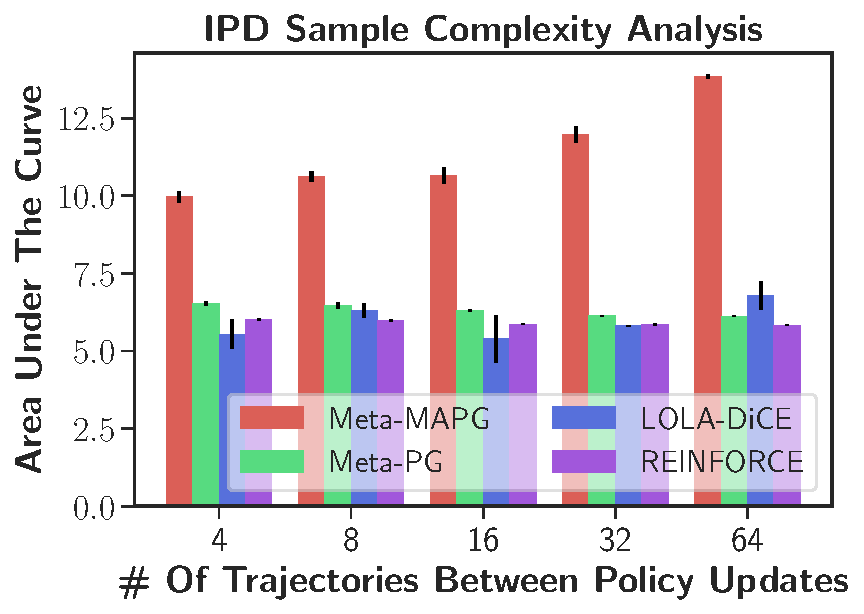
\includegraphics[height=2.9cm]{figs/sample_complexity.pdf}
        \caption{}
        \label{fig:sample-complexity}
    \end{subfigure}
    \begin{subfigure}[b]{0.247\linewidth}
        \centering
        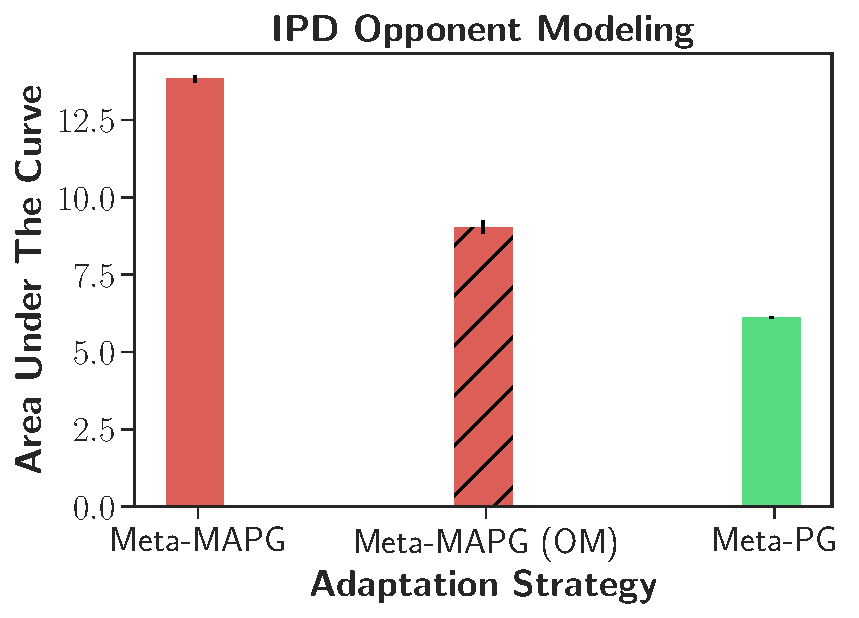
\includegraphics[height=2.9cm]{figs/ipd_om.pdf}
        \caption{}
        \label{fig:ipd-om}
    \end{subfigure}
    \begin{subfigure}[b]{0.247\linewidth}
        \centering
        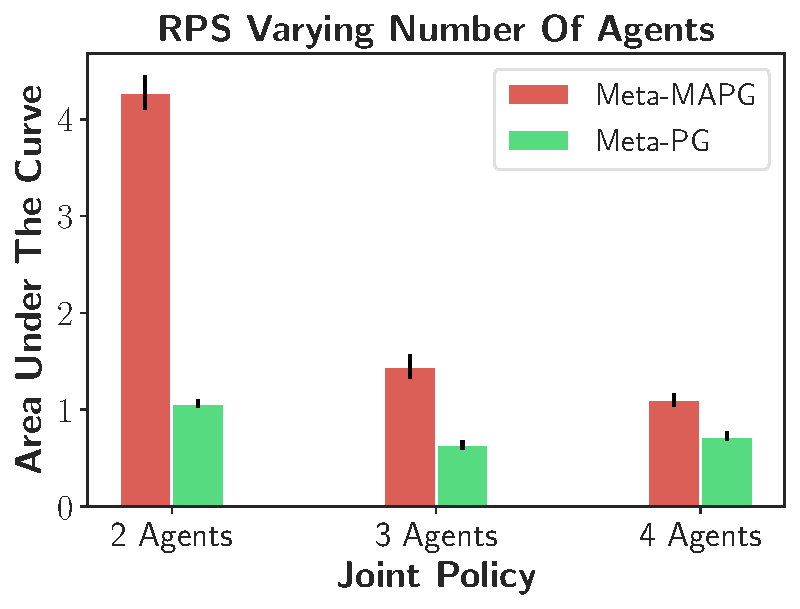
\includegraphics[height=2.9cm]{figs/rps_number.pdf}
        \caption{}
        \label{fig:rps-number}
    \end{subfigure}
    \begin{subfigure}[b]{0.247\linewidth}
        \centering
        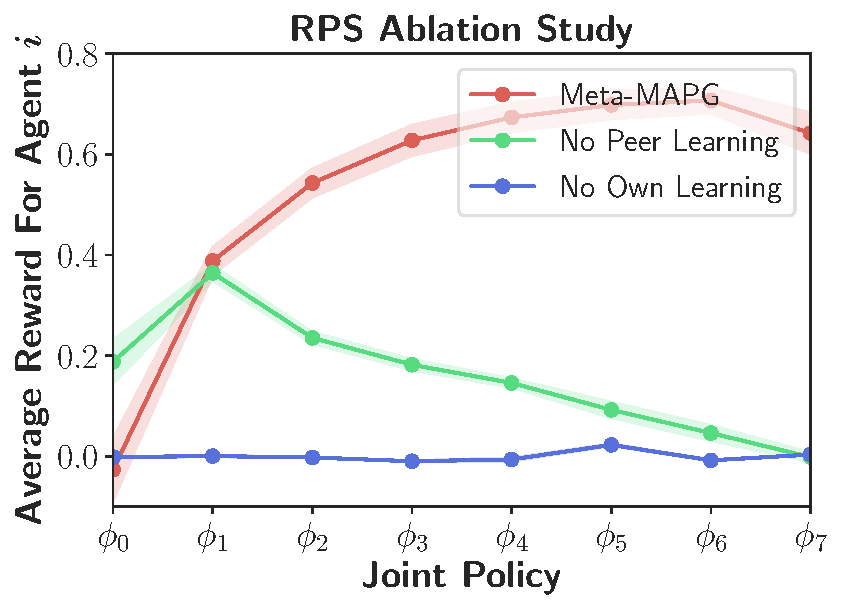
\includegraphics[height=2.9cm]{figs/rps_abb.pdf}
        \caption{}
        \label{fig:rps-abb}
    \end{subfigure}
    \vspace{-0.9cm}
    \caption{
    (\textbf{a}) Adaptation performance with a varying number of trajectories. Meta-MAPG's performance generally improves with a larger $K$. (\textbf{b}) Adaptation performance with opponent modeling. Meta-MAPG with OM computes the peer learning gradient in a decentralized manner. (\textbf{c}) Adaptation performance with a varying number of agents, where Meta-MAPG achieves the best AUC in all cases.
    (\textbf{d}) Ablation study for Meta-MAPG. Meta-MAPG achieves significantly better performance than the two ablated baselines. 
    }
    \vskip-0.17in
\end{figure*}
%%%%%%%%%%%%%%%%%%%%%%%%%%%%%%

\subsection{RPS Environment: Competitive}
\begin{question}
How effective is Meta-MAPG in a fully competitive scenario? \\[-2em]
\end{question}
We have demonstrated the benefit of our approach in the mixed incentive scenario of IPD. Here, we consider another classic iterated game, rock-paper-scissors (RPS) with a fully competitive payoff table (see \cref{tab:rps-payoff-table}). 
In RPS, at each time step agents $i$ and $j$ can choose an action of either (R)ock, (P)aper, or (S)cissors. The state space is defined as $s_{0}\!=\!\varnothing$ and $s_{t}\!=\!\bm{a}_{\bm{t-1}}$ for $t\geq1$.
For meta-learning, we consider a population of initial personas $p(\bm{\phi}^{\bm{-i}}_{\bm{0}})$, including the rock/paper/scissors persona (with a rock/paper/scissors actions probability between $1/3$ and $1$).
% As in IPD, an agent $j$ is initialized randomly from the population and updates its policy while interacting with $i$.

\cref{fig:rps-result} shows the adaptation performance during meta-testing.
Similar to the IPD results, we observe that the baseline methods have effectively converged to win against the opponent $j$ in the first few trajectories. For instance, agent $i$ has a high rock probability when playing against $j$ with a high initial scissors probability (see \cref{fig:rps-meta-pg-analysis,fig:rps-dice-analysis,fig:rps-reinforce-analysis} in Appendix). 
This strategy, however, results in the opponent quickly changing its behavior toward the mixed Nash equilibrium strategy of $(1/3, 1/3, 1/3)$ for the rock, paper, and scissors probabilities.
In contrast, our meta-agent learned to lose slightly in the first two trajectories $\tau_{\bm{\phi}_{\bm{0:1}}}$ to achieve much larger rewards in the later trajectories $\tau_{\bm{\phi}_{\bm{2:7}}}$ while relying on its ability to adapt more efficiently than its opponent (see~\cref{fig:rps-meta-mapg-analysis} in Appendix).
Compared to the IPD results, we observe that it is more difficult for our meta-agent to shape $j$'s future policies in RPS possibly due to the fact that RPS has a fully competitive payoff structure, while IPD has a mixed incentive structure.

\begin{question}
How effective is Meta-MAPG in settings with more than one peer?
\\[-2em]
\end{question}
Our meta-multiagent policy gradient theorem is general and can be applied to scenarios with more than one peer.
To validate this, we experiment with 3-player and 4-player RPS, where we consider sampling peers randomly from the entire persona population. 
We note that the domain becomes harder as the number of agents $n$ increases, because the state space dimension grows exponentially as a function of $n$ and a meta-agent needs to consider more peers in shaping their future policies. 
\Cref{fig:rps-number} shows a comparison against the Meta-PG baseline. 
We generally observe that the peer agents change their policies toward the mixed Nash equilibrium more quickly as the number of agents increases, which results in decreased performance for all methods. 
Nevertheless, Meta-MAPG achieves the best performance in all cases and can clearly be easily extended to settings with a greater number of agents.
% \dXX{todo: payoff table specify}

\begin{question}
What happens if a meta-agent is trained without the own learning gradient?
\\[-2em]
\end{question}
Our meta-multiagent policy gradient theorem inherently includes both the own learning and peer learning gradient, but is it necessary to have both terms?
To answer this question, we conduct an ablation study and compare Meta-MAPG to two methods: one trained without the peer learning gradient and another trained without the own learning gradient. 
Note that not having the peer learning term is equivalent to Meta-PG, and not having the own learning term is similar to LOLA-DiCE but alternatively trained with a meta-optimization procedure. \Cref{fig:rps-abb} shows that a meta-agent trained without the peer learning term cannot properly exploit the peer agent's learning process. 
Also, a meta-agent trained without the own learning term cannot change its own policy effectively in response to anticipated learning by peer agents.
By contrast, Meta-MAPG achieves superior performance by accounting for both its own learning process and the learning processes of peer agents.

\subsection{2-Agent HalfCheetah Environment: Cooperative}
\begin{question}
Does considering the peer learning gradient always improve performance? \\[-2em]
\end{question}
To answer this question, we experiment with a fully cooperative setting of the the 2-Agent HalfCheetah domain~\citep{dewitt2020deep_multimujoco}, where the first and second agent control three joints of the back and front leg with continuous action spaces, respectively (see~\cref{fig:multi-mujoco-domain}). 
Both agents receive a joint reward corresponding to making the cheetah robot run to the right as soon as possible.
Note that two agents are coupled \textit{within} the cheetah robot, requiring close cooperation and coordination between them.

For meta-learning, we consider a population of teammates with varying degrees of expertise in running to the \textit{left} direction. 
Specifically, we pre-train a teammate $j$ and build a population based on checkpoints of its parameters during learning. 
\Cref{fig:mujoco-teammate-vis} in Appendix shows the distribution of $j$'s expertise. Note that we construct the distribution with a significant gap to ensure that the meta-testing distribution is sufficiently different from the meta-training/validation distribution. This allows us to effectively evaluate the ability of our approach to generalize its learning.
During meta-learning, $j$ is randomly initialized from this population of policies. 
Importantly, $j$ must adapt its behavior in this setting because the agent has achieved the \textit{opposite} skill during pre-training compared to the true objective of moving to the right. 
Hence, a meta-agent $i$ should succeed by both adapting to differently initialized teammates with varying expertise in moving the opposite direction, and guiding $j$'s learning process to coordinate the eventual right movement. 

Our results are displayed in~\cref{fig:halfcheeta-result-finale}. There are two notable observations. First, influencing peer learning does not help much in cooperative settings and Meta-MAPG performs similarly to Meta-PG.
The peer learning gradient attempts to shape the future policies of other agents so that the meta-agent can take advantage. In IPD, for example, the meta-agent influenced $j$ to be cooperative in the future such that the meta-agent can act with a high probability of the defect action and receive higher returns. 
However, in cooperative settings, due to the joint reward, $j$ is already changing its policies in order to benefit the meta-agent, resulting in a less significant effect with respect to the peer learning gradient. 
Second, Meta-PG and Meta-MAPG outperform the other approaches of LOLA-DiCE and REINFORCE, achieving higher rewards when interacting with a new teammate. 

% %%%%%%%%%%%%%%%%%%%%%%%%%%%%%%%%
% \begin{figure}[t]
%     \centering
%     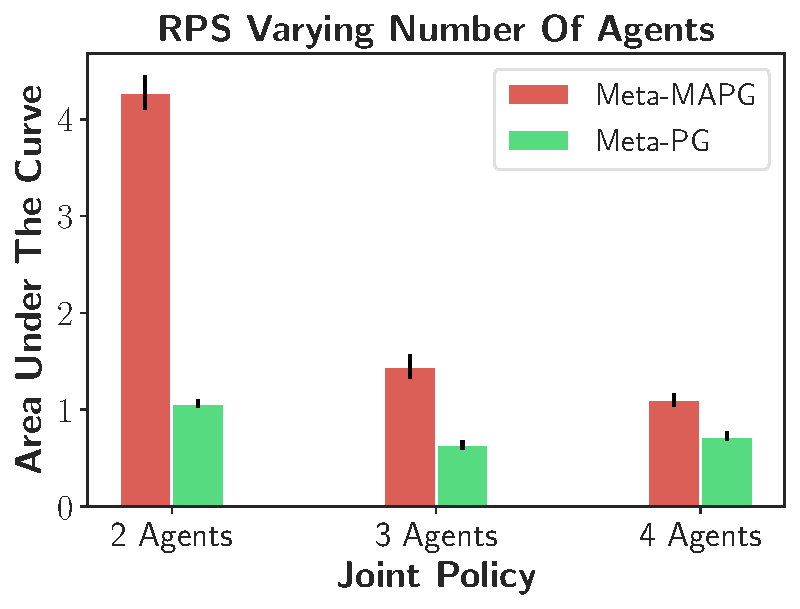
\includegraphics[height=3.1cm]{figs/rps_number.pdf}
%     \caption{
% Adaptation performance with a varying number of agents in RPS, where Meta-MAPG achieves the best AUC in all cases.}
%     \label{fig:rps-number}
% \end{figure}
% %%%%%%%%%%%%%%%%%%%%%%%%%%%%%%%%
% %%%%%%%%%%%%%%%%%%%%%%%%%%%%%%%%
% \begin{figure}[t]
%     \centering
%     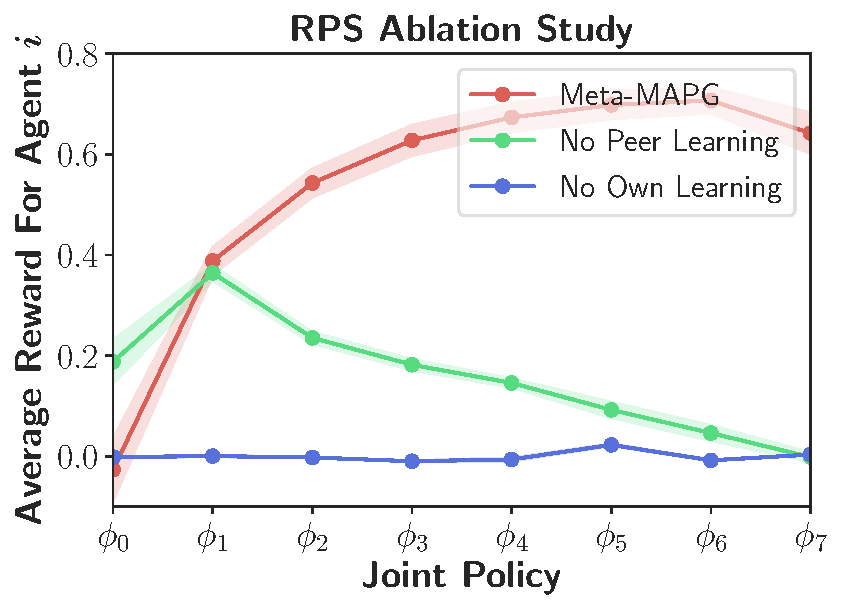
\includegraphics[height=3.1cm]{figs/rps_abb.pdf}
%     \caption{
% Ablation study for Meta-MAPG. Meta-MAPG achieves significantly better performance than ablated baselines with no own learning gradient and no peer learning gradient.}
%     \label{fig:rps-abb}
% \end{figure}
% %%%%%%%%%%%%%%%%%%%%%%%%%%%%%%%%